% !TeX program = xelatex
\documentclass[12pt,a4paper]{article}

\usepackage{fontspec}
\usepackage[english]{babel}
\usepackage{amsmath,amssymb}
\usepackage{geometry}
\usepackage{tikz}
\usepackage{xcolor}
\usepackage{enumitem}
\usepackage{booktabs}
\setmainfont{Latin Modern Roman}

\geometry{margin=2.5cm}

\definecolor{TitleColor}{HTML}{0B3C5D}
\definecolor{QuestionColor}{HTML}{0D3B66}
\definecolor{ChoiceColor}{HTML}{8A2D12}

\renewcommand{\labelenumi}{\textbf{\color{QuestionColor}\arabic{enumi}.}}
\renewcommand{\labelenumii}{\textbf{\color{ChoiceColor}(\alph{enumii})}}

\setlist[enumerate,1]{leftmargin=*,font=\bfseries\color{QuestionColor}}
\setlist[enumerate,2]{leftmargin=1.2cm,font=\bfseries\color{ChoiceColor}}
\setlist[itemize]{leftmargin=1.2cm,font=\bfseries\color{ChoiceColor},label=\textbf{\color{ChoiceColor}$\blacktriangleright$}}

\title{\textbf{\color{TitleColor}Probability and Statistics for Engineers MAT204\\[0.3cm]
Reinforcement Exercise 2 -- Solutions}}
\author{}
\date{}

\begin{document}
\maketitle

\section*{\textbf{\color{TitleColor}Answers}}

\begin{enumerate}

%--------------------------------------------------------------------
% QUESTION 1 — Expected Value
%--------------------------------------------------------------------
\item When two dice are rolled, the total sample space is $|S|=36$.

\textbf{Definition of the events:}
\[
A=\text{``at least one die shows 4''},\qquad B=\text{``pairs whose sum is 7''}.
\]

\textbf{Probability of event $A$} (using the complement):
\[
P(A)=1-P(\text{no die shows 4})=1-\frac{5}{6}\cdot\frac{5}{6}=1-\frac{25}{36}=\frac{11}{36}.
\]

\textbf{Probability of event $B$} ($(1,6),(2,5),(3,4),(4,3),(5,2),(6,1)$ have sum $7$):
\[
P(B)=\frac{6}{36}=\frac{1}{6}.
\]

\textbf{Intersection $A\cap B$} (both sum $7$ and at least one die is $4$: $(4,3)$ and $(3,4)$):
\[
P(A\cap B)=\frac{2}{36}.
\]

\textbf{Probability of winning} (inclusion-exclusion):
\[
P(K)=P(A)+P(B)-P(A\cap B)=\frac{11}{36}+\frac{6}{36}-\frac{2}{36}=\frac{15}{36}=\frac{5}{12}.
\]

\textbf{Probability of losing:}
\[
P(L)=1-\frac{5}{12}=\frac{7}{12}.
\]

\begin{center}
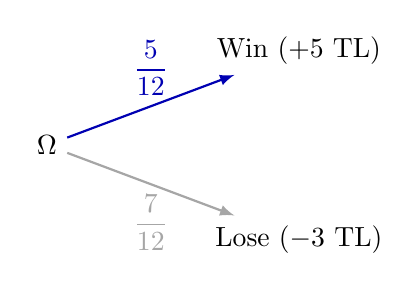
\begin{tikzpicture}[>=latex, line width=0.8pt]
  \node (om) at (0,0) {$\Omega$};
  \node (k)  at (3.2, 1.2) {Win ($+5$~TL)};
  \node (l)  at (3.2,-1.2) {Lose ($-3$~TL)};
  \draw[->,blue!70!black] (om) -- (k) node[midway,above] {$\dfrac{5}{12}$};
  \draw[->,gray!70]       (om) -- (l) node[midway,below] {$\dfrac{7}{12}$};
\end{tikzpicture}
\end{center}

\begin{enumerate}
\item Expected value for a single game:
\[
E(X)=5\cdot\frac{5}{12}+(-3)\cdot\frac{7}{12}=\frac{25}{12}-\frac{21}{12}=\frac{4}{12}=\frac{1}{3}\ \text{TL}.
\]
\[
{\color{red}\boxed{E(X)=\frac{1}{3}\ \text{TL}\approx 0.33\ \text{TL}}}
\]

\item Expected total gain for $10$ games:
\[
10\cdot E(X)=10\cdot\frac{1}{3}=\frac{10}{3}\ \text{TL}.
\]
When the entry fee ($30$~TL) is subtracted, the net expected value is:
\[
\frac{10}{3}-30=\frac{10-90}{3}=-\frac{80}{3}\ \text{TL}\approx -26.67\ \text{TL}.
\]
\[
{\color{red}\boxed{\text{Net expected gain}=-\frac{80}{3}\ \text{TL}\approx -26.67\ \text{TL}}}
\]
\end{enumerate}

%--------------------------------------------------------------------
% QUESTION 2 — Discrete Random Variable / CDF
%--------------------------------------------------------------------
\item The given probabilities (grades are ordered from worst to best) are:
\[
P(F)=0.15,\quad
P(E)=0.03,\quad
P(D)=0.07,\quad
P(C)=0.25,\quad
P(B)=0.32,\quad
P(A)=0.18.
\]

\begin{enumerate}
\item Cumulative distribution function (CDF) table:

\begin{center}
\begin{tabular}{ccc}
\toprule
\textbf{Grade} & $P(X=x)$ & $F(x)=P(X\le x)$\\
\midrule
F & $0.15$ & $0.15$\\
E & $0.03$ & $0.18$\\
D & $0.07$ & $0.25$\\
C & $0.25$ & $0.50$\\
B & $0.32$ & $0.82$\\
A & $0.18$ & $1.00$\\
\bottomrule
\end{tabular}
\end{center}

\item Getting a grade higher than B means receiving only grade A:
\[
P(X>B)=P(A)=0.18.
\]
\[
{\color{red}\boxed{P(X>B)=0.18}}
\]

\item Getting a grade lower than C means receiving D, E, or F:
\[
P(X<C)=P(D)+P(E)+P(F)=0.07+0.03+0.15=0.25.
\]
\[
{\color{red}\boxed{P(X<C)=0.25}}
\]
\end{enumerate}

%--------------------------------------------------------------------
% QUESTION 3 — Total Probability and Bayes' Theorem (Robot Source)
%--------------------------------------------------------------------
\item Given:
\[
P(A)=0.60,\qquad P(B)=0.40,
\]
\[
P(H\mid A)=0.05,\qquad P(H\mid B)=0.10.
\]

\begin{center}
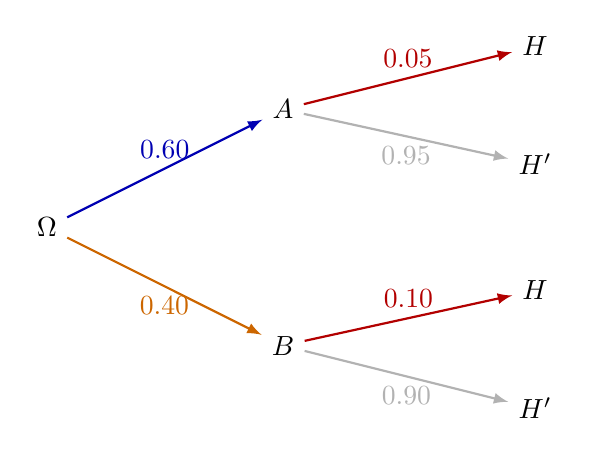
\begin{tikzpicture}[>=latex, line width=0.8pt]
  \node (om) at (0,0) {$\Omega$};
  \node (ra) at (3.0, 1.5) {$A$};
  \node (rb) at (3.0,-1.5) {$B$};
  \node (ha) at (6.2, 2.3) {$H$};
  \node (hac) at (6.2, 0.8) {$H'$};
  \node (hb) at (6.2,-0.8) {$H$};
  \node (hbc) at (6.2,-2.3) {$H'$};

  \draw[->,blue!70!black]  (om) -- (ra)   node[midway,above] {$0.60$};
  \draw[->,orange!80!black](om) -- (rb)   node[midway,below] {$0.40$};
  
  \draw[->,red!70!black]   (ra) -- (ha)   node[midway,above] {$0.05$};
  \draw[->,gray!60]        (ra) -- (hac)  node[midway,below] {$0.95$};
  \draw[->,red!70!black]   (rb) -- (hb)   node[midway,above] {$0.10$};
  \draw[->,gray!60]        (rb) -- (hbc)  node[midway,below] {$0.90$};
\end{tikzpicture}
\end{center}

\begin{enumerate}
\item \textbf{Total defect probability $P(H)$:} \\
A defective part must have come from either A or B:
\[
P(H)=P(H\mid A)P(A)+P(H\mid B)P(B)
\]
\[
P(H)=0.05\cdot0.60+0.10\cdot0.40=0.030+0.040=0.070.
\]
\[
{\color{red}\boxed{P(H)=0.07}}
\]

\item \textbf{$P(B\mid H)$ using Bayes' theorem:} \\
The probability that a known defective part came from B is:
\[
P(B\mid H)=\frac{P(H\mid B)\,P(B)}{P(H)}=\frac{0.10\cdot0.40}{0.070}=\frac{0.040}{0.070}=\frac{4}{7}\approx 0.5714.
\]
\[
{\color{red}\boxed{P(B\mid H)=\frac{4}{7}\approx 0.5714}}
\]
\end{enumerate}

%--------------------------------------------------------------------
% QUESTION 4 — Continuous Random Variable / PDF and CDF
%--------------------------------------------------------------------
\item The probability density function is:
\[
f(x)=c(x+1),\qquad 1<x<3.
\]

\begin{enumerate}
\item \textbf{Finding the constant $c$} (normalization condition):
\[
\int_{1}^{3}f(x)\,dx=1
\quad\Rightarrow\quad
c\int_{1}^{3}(x+1)\,dx=1.
\]
Evaluating the integral:
\[
\int_{1}^{3}(x+1)\,dx=\left[\frac{x^2}{2}+x\right]_{1}^{3}
=\left(\frac{9}{2}+3\right)-\left(\frac{1}{2}+1\right)=\frac{15}{2}-\frac{3}{2}=6.
\]
Therefore:
\[
6c=1\quad\Rightarrow\quad c=\frac{1}{6}.
\]
\[
{\color{red}\boxed{c=\frac{1}{6}}}
\]

\item \textbf{Distribution function $F(x)$:}
\[
F(x)=\int_{1}^{x}\frac{1}{6}(t+1)\,dt
=\frac{1}{6}\left[\frac{t^2}{2}+t\right]_{1}^{x}
=\frac{1}{6}\left(\frac{x^2}{2}+x-\frac{3}{2}\right)
=\frac{x^2+2x-3}{12}.
\]
\[
{\color{red}\boxed{F(x)=
\begin{cases}
0, & x\le 1,\\[4pt]
\dfrac{x^2+2x-3}{12}, & 1<x<3,\\[4pt]
1, & x\ge 3.
\end{cases}}}
\]
\end{enumerate}

%--------------------------------------------------------------------
% QUESTION 5 — Conditional Probability and Bayes (Cancer Test)
%--------------------------------------------------------------------
\item Given:
\[
P(C)=0.05,\qquad P(C^c)=0.95,
\]
\[
P(+\mid C)=0.78,\qquad P(+\mid C^c)=0.06.
\]

\begin{center}
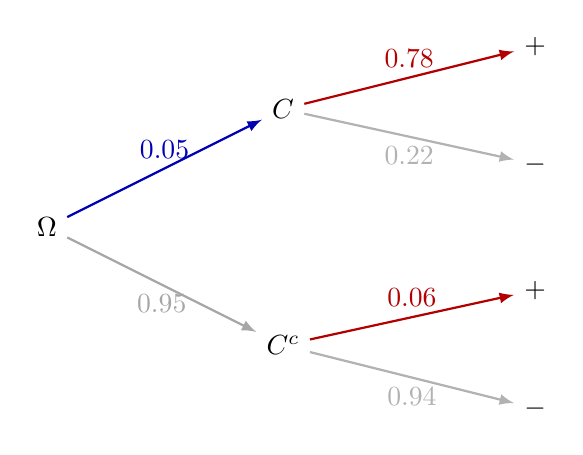
\begin{tikzpicture}[>=latex, line width=0.8pt]
  \node (om) at (0,0) {$\Omega$};
  \node (c)  at (3.0, 1.5) {$C$};
  \node (cc) at (3.0,-1.5) {$C^c$};
  \node (cp) at (6.2, 2.3) {$+$};
  \node (cn) at (6.2, 0.8) {$-$};
  \node (ccp) at (6.2,-0.8) {$+$};
  \node (ccn) at (6.2,-2.3) {$-$};

  \draw[->,blue!70!black]  (om) -- (c)   node[midway,above] {$0.05$};
  \draw[->,gray!70]        (om) -- (cc)  node[midway,below] {$0.95$};
  \draw[->,red!70!black]   (c)  -- (cp)  node[midway,above] {$0.78$};
  \draw[->,gray!60]        (c)  -- (cn)  node[midway,below] {$0.22$};
  \draw[->,red!70!black]   (cc) -- (ccp) node[midway,above] {$0.06$};
\draw[->,gray!60]        (cc) -- (ccn) node[midway,below] {$0.94$};
\end{tikzpicture}
\end{center}

\textbf{Total probability of a positive test:}
\[
P(+)=P(+\mid C)\,P(C)+P(+\mid C^c)\,P(C^c)
=0.78\cdot0.05+0.06\cdot0.95
=0.039+0.057=0.096.
\]

\textbf{Applying Bayes' theorem:}
\[
P(C\mid +)=\frac{P(+\mid C)\,P(C)}{P(+)}=\frac{0.78\cdot0.05}{0.096}=\frac{0.039}{0.096}\approx 0.4063.
\]
\[
{\color{red}\boxed{P(C\mid +)\approx 0.4063}}
\]

This result shows that even if the test is positive, the probability of actually having cancer is only about 40.6\%. The low prevalence of the disease in the population ($P(C)=0.05$) makes this value smaller than one might expect.

\end{enumerate}

\vspace{1cm}
\section*{\textbf{\color{TitleColor}Just Think: Hard Question (Not Graded) -- Solution}}

In a population, each family's childbearing behavior is modeled as follows: At each birth, the probability that the child is a boy or a girl is equal, so
\[
P(\text{Boy}) = P(\text{Girl}) = \frac{1}{2}
\]
holds. Each family continues to have children until the first boy is born; once the first boy is born, the family stops having children.

\begin{enumerate}
    \item[\textbf{a)}] \textbf{Sample Space:} $S = \{B, GB, GGB, \dots\}$. Since it can continue indefinitely and its elements can be listed one by one, it is discrete and countably infinite.
    
    \item[\textbf{b)}] \textbf{PMF:} Let $X$ be the number of girls. This is the number of failures (girls) before the first success with probability $p=1/2$ (boy), so it follows a geometric distribution:
    \[
    P(X=x) = \left(\frac{1}{2}\right)^x \cdot \frac{1}{2} = \left(\frac{1}{2}\right)^{x+1}, \quad x=0, 1, 2, \dots
    \]
    
    \item[\textbf{c)}] \textbf{Expected Value:} For a geometric distribution, $E(X) = \frac{1-p}{p}$, so $E(X) = \frac{1/2}{1/2} = 1$. The expected number of girls is $1$.
    
    \item[\textbf{d)}] \textbf{Comparison:} Since each family stops after having one boy, the expected number of boys is $1$. The expected number of girls is also $1$. Therefore, the two values are \textbf{equal}.
    
    \item[\textbf{\color{ChoiceColor}e)}] \textcolor{ChoiceColor}{\textbf{Interpretation: Since each family has an average of 1 girl and 1 boy, the long-run girl/boy ratio in the population does not change; it remains 1:1.}}
\end{enumerate}

\end{document}
